\section{Background Theory}
The following section covers theory falls outside of common knowledge of that studied by a student undertaking a Mechanical Engineering degree at UNSW. It includes detail on ADS-B, CubeSat design and Satellite Constellation design.
\subsection{Automatic Dependant Surveillance-Broadcast (ADS-B)}
ADS-B is an aircraft tracking system based upon digital aircraft-to-ground and aircraft-to-aircraft transmissions.  It is intended to support the existing Air Traffic Control Radar Beacon System (ATCRBS) which uses radar to track aircraft. ADS-B is now being adopted as a primary ATC management system in the United States of America \cite{ADSB_DOT}, the European Union and Australia \cite{ADSB_CASA_booklet}. 

\subsubsection{Data Structure}
ADS-B systems expand upon the function provided by Secondary Surveillance Radar (SSR) by requiring that extra data be periodically broadcast by all aircraft, without interrogation. The expanded data set includes Global Navigation Satellite System (GNSS) positioning and emergency telemetry. The ADS-B standard requires an update rate of once every second.

Current ADS-B systems use the GNSS data acquired by on-board avionics for position determination \cite{ADSB_ICAO_man}. This data is transmitted to ground ATC stations and shared between aircraft in order to allow for accurate tracking of aircraft position for both ATC stations and other aircraft in the immediate vicinity. 

ADS-B is also capable of relaying other aircraft telemetry data. As a minimum, the Australian Civil Aviation Safety Authority (CASA) specify the following to be included an an ADS-B data-set  \cite[Clause 8.2.3]{ADSB_AC_specs}:
\begin{itemize}
	\item \textbf{Position} - determined via on-board avionics, including GNSS systems
	\item\textbf{Position Integrity Information} - indicating the level of trust with the positioning data
	\item \textbf{Pressure Altitude} - the altitude of an aircraft as determined by on-board altimeter
	\item \textbf{Aircraft Identification}
	\item \textbf{Version Number} - the version number and compliancy of the on-board avionics equipment.
\end{itemize}
In addition, the Australian ATC system has specified an additional 'highly desirable' data set \cite[Clause 8.2.4]{ADSB_AC_specs}:
\begin{itemize}
	\item \textbf{SPI Indication} - Special Position Identification, intended to supplement position data in the initial packet
	\item \textbf{Emergency Flag}
	\item \textbf{Emergency Priority Status Information}
	\item \textbf{Velocity Information}
	\item \textbf{GNSS Height}
	\item \textbf{Vertical Rate}
	\item \textbf{Aircraft category}
\end{itemize}


\subsubsection{Transmission and Modulation}
ADS-B data is intended to be transmitted over either the Universal Access Transceiver Standard UAT), or the 1090MHz Mode S Extended Squitter, previously used by SSR. Specifications for ADS-B over UAT is given in \cite{RTCA_UAT} and over Mode S in \cite{RTCA_MODE_S}. ADS-B is broadcast on a random-access basis with particular aircraft identified by information in their data packets \cite{Blomenhofer2012}.

\subsubsection{Coverage}
Tracking via ADS-B requires aircraft to be within the line-of-sight of a ground station \cite{ADSB_CASA_booklet}. ADS-B coverage areas vary with altitude and the existence of obstructing features in the terrain surrounding a ground station. Australia is one of the earliest adopters of ADS-B technology, with coverage over 100 percent of Australia's landmass as shown in Figure \ref{fig:adsb_aus_coverage} \cite{ADSB_CASA_booklet}.
\begin{figure}[H]
	\centering
	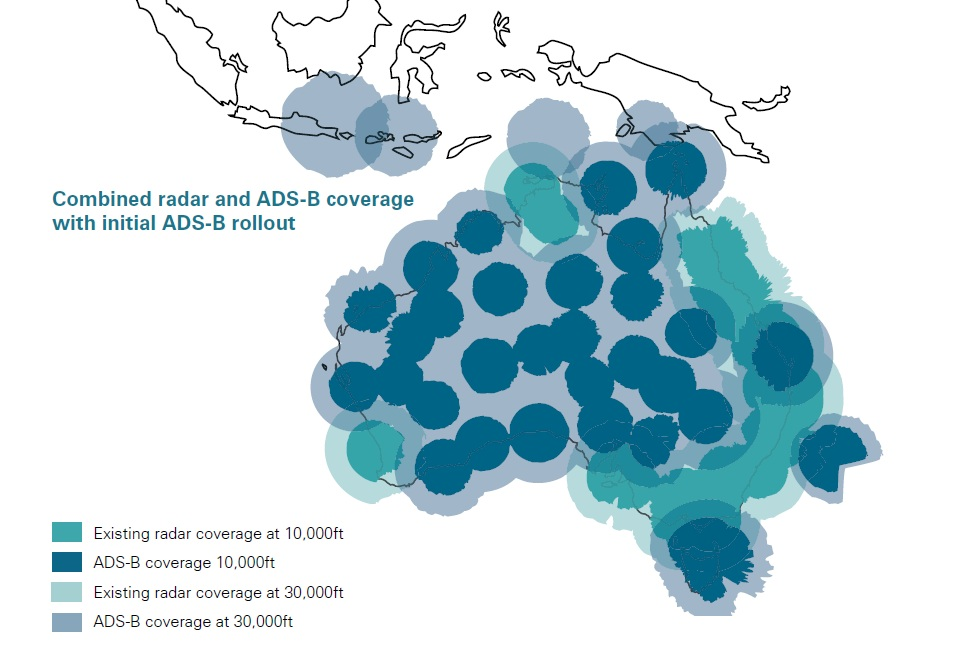
\includegraphics[scale = 0.5]{Pictures/adsb_coverage.jpg}
	
	\caption[ADS-B and radar coverage in Australia]{ADS-B and radar coverage in Australia, reproduced from \cite{ADSB_CASA_booklet}}
	\label{fig:adsb_aus_coverage}
\end{figure}

Out of the range of these ground stations, aircraft tracking via ADS-B is not possible.  Although comprehensive coverage is currently being implemented in Australia \cite{ADSB_CASA_booklet}, the Asia-Pacific region \cite{ADSB_ICAO_man} and much of North America \cite{ADSB_DOT}, there still exists areas, particularly over oceanic and polar regions where the service is not available. Figure \ref{fig:adsb_us_coverage} shows the state of ADS-B coverage in US as of 30/06/2013.
\begin{figure}[H]
	\centering
	\includegraphics[scale = 0.5]{Pictures/adsb_coverage_US.jpg}
	
	\caption[ADS-B coverage in the US as of 30/06/2013]{ADS-B coverage in the US as of 30/06/2013, reproduced from \cite{NextGEN_coverage_map}}
	\label{fig:adsb_us_coverage}
\end{figure}
Some solutions exist for ADS-B coverage in remote and marine areas. Areas where ADS-B is not adequately covered is illustrated in Figure \ref{fig:adsb_nocoverage}, as  estimated by \cite{ADS-B:Aireon_brochure}. Ground stations installed on oil platforms currently provide coverage over the Gulf of Mexico \cite{ADSB_DOT}. Both Globalstar \cite{ADS-B:Globalstar_webinar} and Iridium NEXT \cite{ADS-B:Aireon_brochure} propose global coverage via Low Earth Orbit (LEO) satellite constellations to be launched in 2014.
\begin{figure}[H]
	\centering
	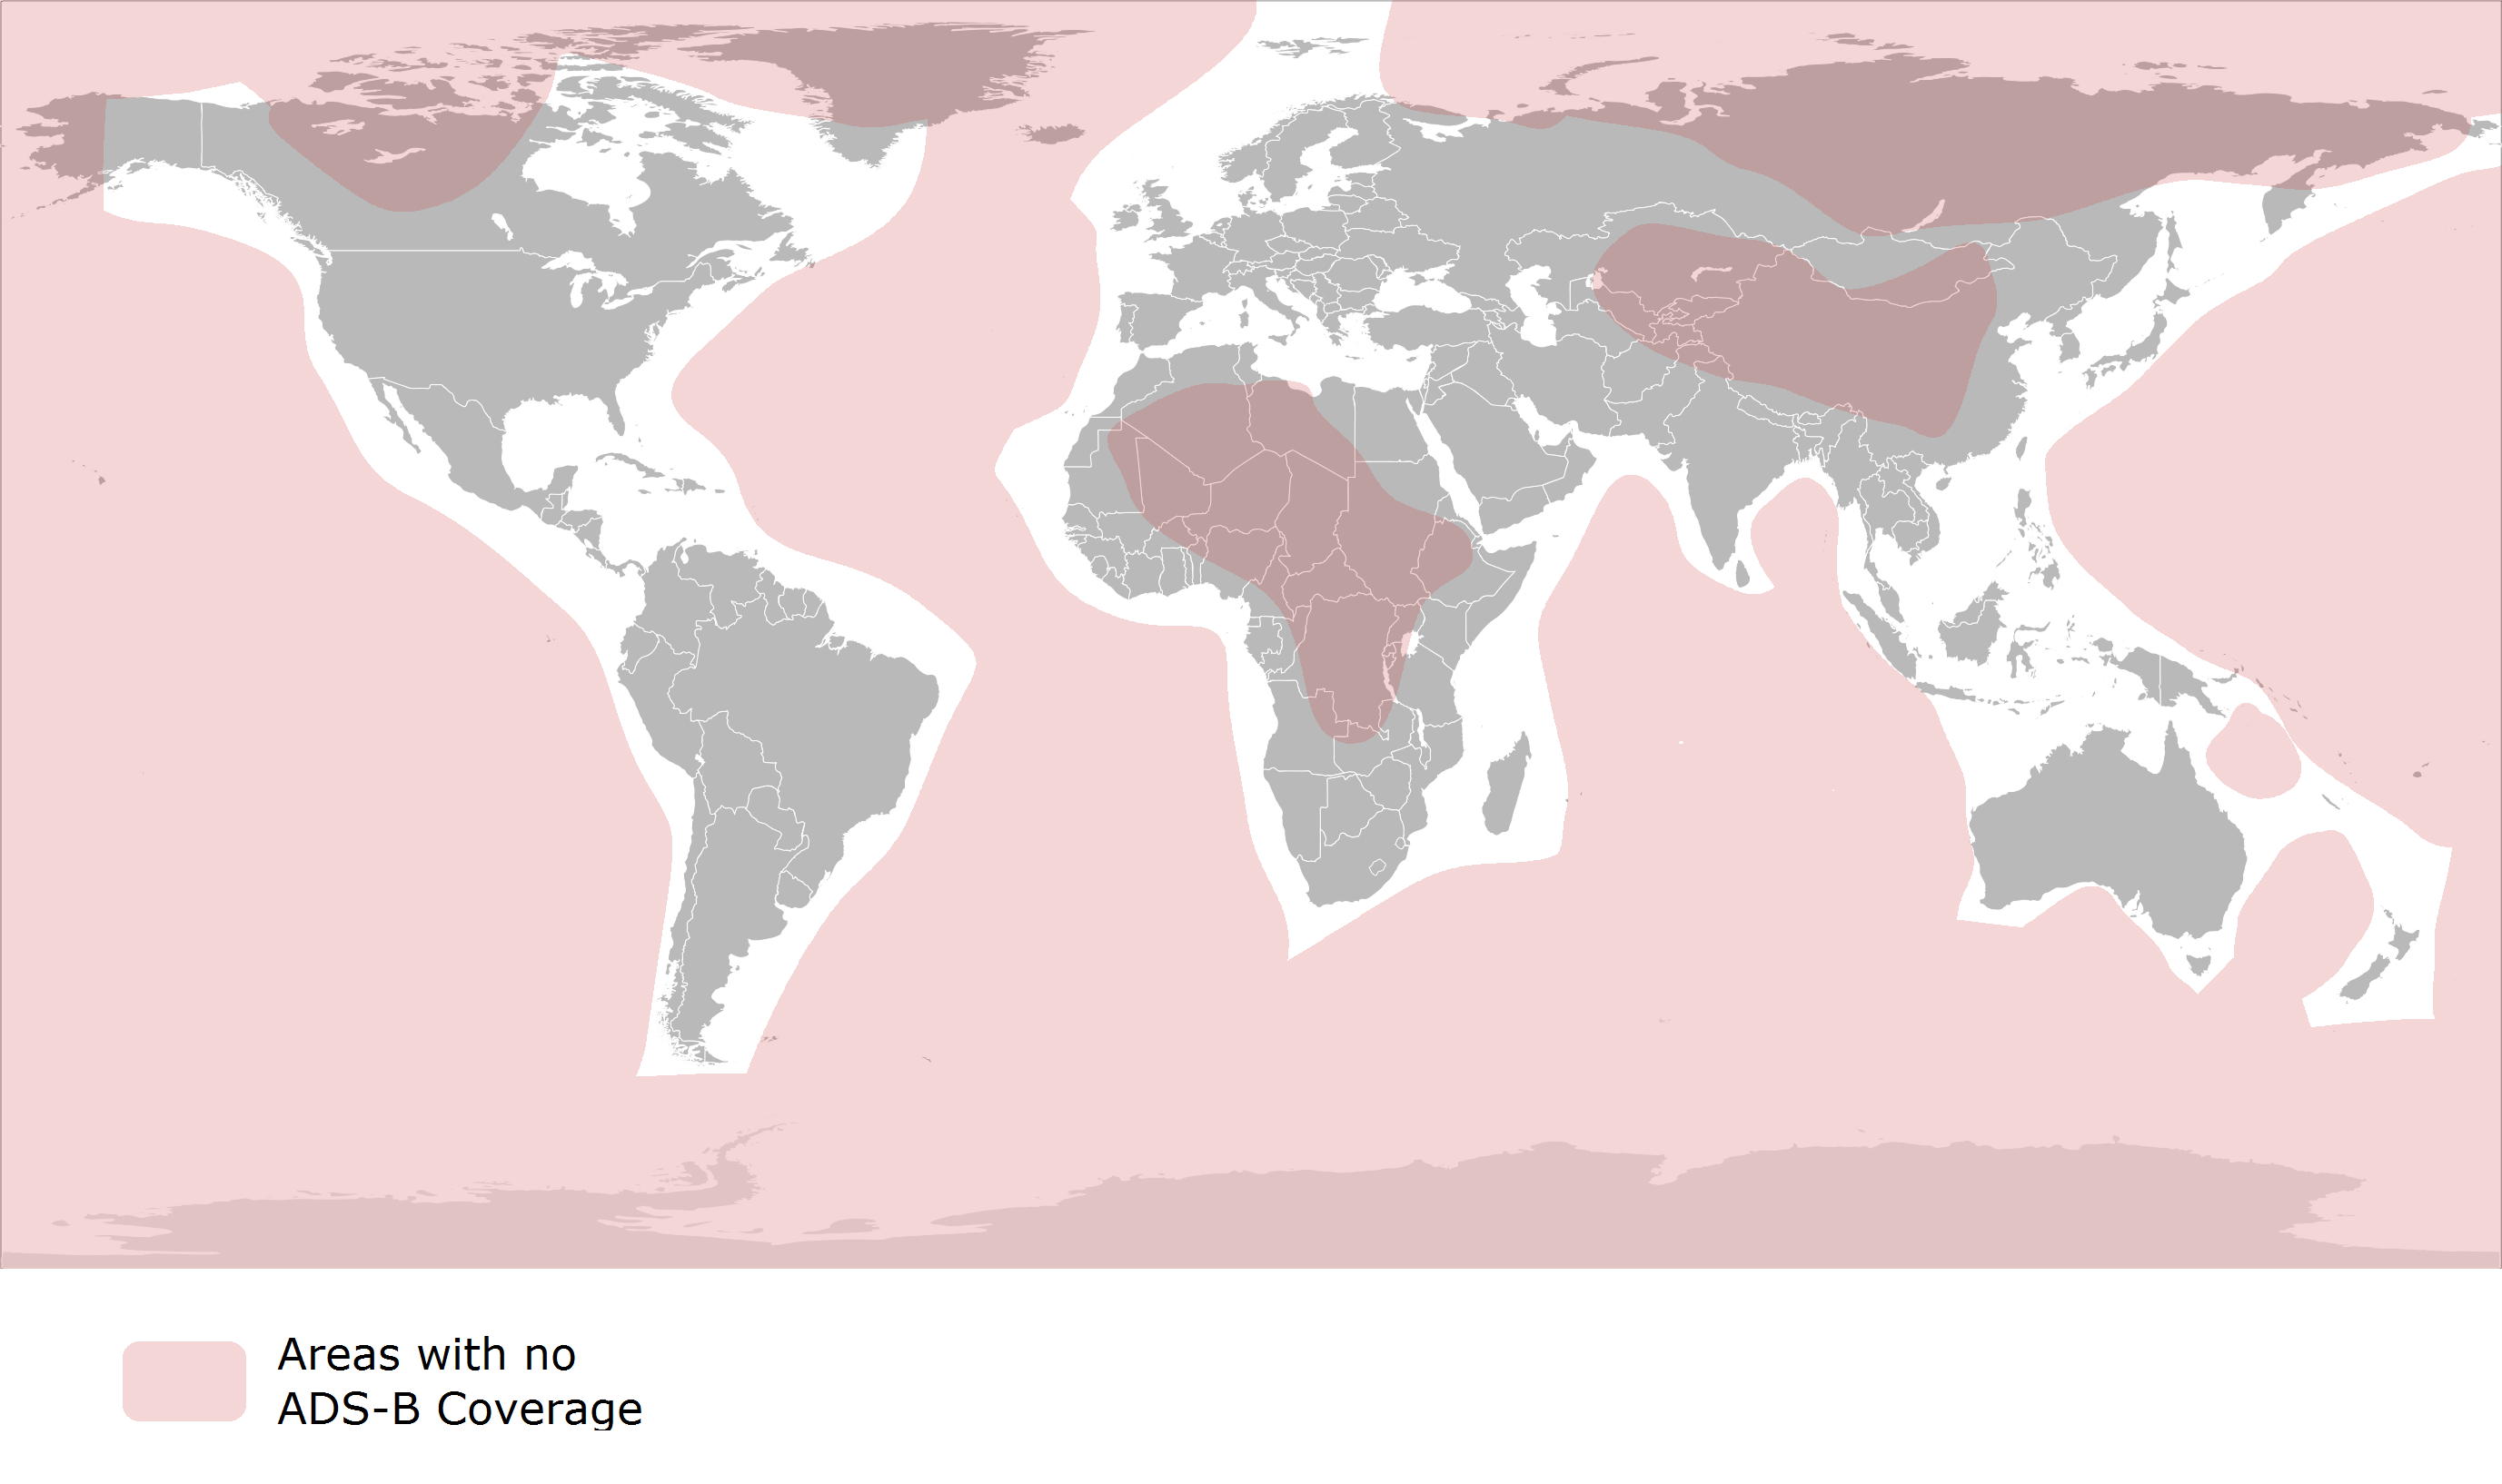
\includegraphics[scale = 0.23]{Pictures/adsb_nocoverage.png}
	
	\caption[Global areas without ADS-B coverage]{Global areas without ADS-B coverage, as estimated by \cite{ADS-B:Aireon_brochure}}
	\label{fig:adsb_nocoverage}
\end{figure}

\newpage
\subsection{Cubesats}
CubeSats are a family of pico-satellites whose mechanical and launch-interface subsystems conform to an open-source standard \cite{Lee2011}. These satellites are characterised by the number of `units' they contain. Each `unit' defines a roughly 100$\times$100$\times$100mm cube-shaped physical envelope and a 1kg maximum weight. Satellites with multiple `units' have a greater mass and payload volume budget. An example of a 2-unit (2U) CubeSat is shown in Figure \ref{fig:2U_example}.

\begin{figure}[H]
	\centering
	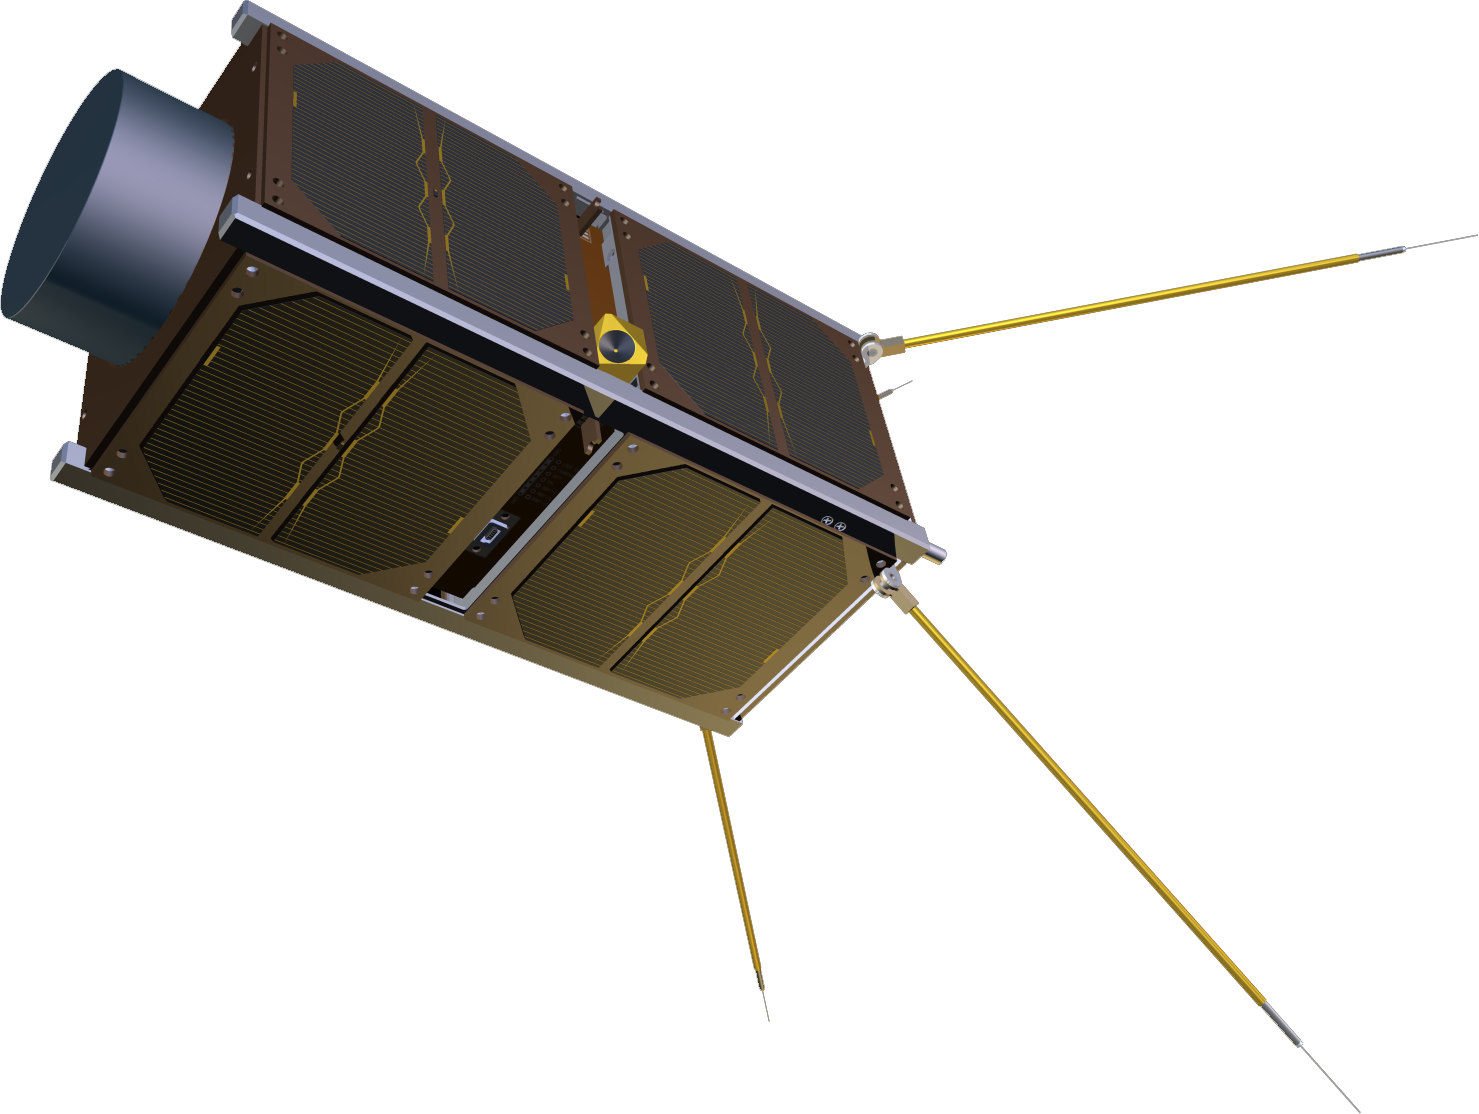
\includegraphics[scale = 0.2]{Pictures/QB50-platform.png}
	
	\caption{The GOMSpace QB50 Platform - an example of a 2U CubeSat, reproduced from \cite{GomSpace2013}}
	\label{fig:2U_example}
\end{figure}

The size and standardisation of CubeSat design have made them accessible to non-military and non-commercial space interest groups, including academic and hobbyist groups. The launch interface design is such that multiple CubeSats can be launched on the same vehicle at reduced cost \cite{Nason2002}. The proliferation of open-source CubeSat designs has allowed the academic and hobbyist community to collaborate and refine CubeSat design concepts. The resulting reduction in design and launch makes developing space-bound payloads more accessible with less risk. Due its reduced size, CubeSats do not have provision for significant orbital manoeuvres and are restricted to LEO missions. 

\subsubsection{Specifications}
Generic CubeSat specifications are given by the California Polytechnic State University (Cal Poly) \cite{Lee2011}. These specifications identify a basic mechanical envelope, materials to be used and a standard launch interface.

Generally, a CubeSat consists of a stacked cube-configuration with 4 rails, each running along the edges of the satellite parallel to the Z axis. Launch and separation switches are located on the bottom face of each of these rails. The design of generic CubeSats is shown in Figure \ref{fig:cubesat_sizes}.

\begin{figure}[htb]
	\centering
	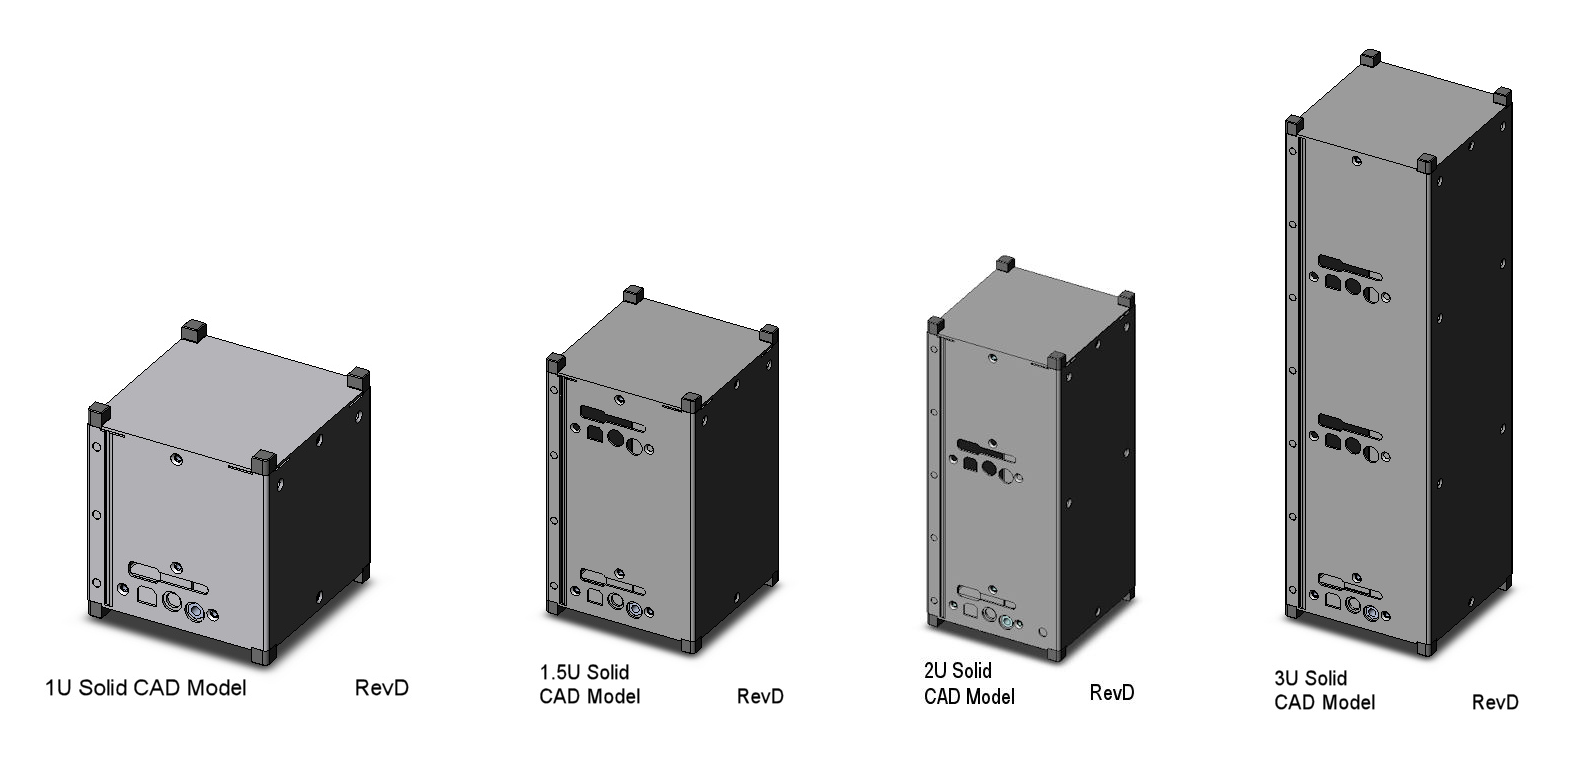
\includegraphics[scale = 0.3]{Pictures/cubesat_sizes.png}
	
	\caption{CubeSat sizes, ranging from the single 1U to the triple 3U. Reproduced from \cite{CubeSatKit2013}}
	\label{fig:cubesat_sizes}
\end{figure}

\subsubsection{Typical Applications}
CubeSats are heavily used by the academic due to their cost-effectiveness and the low-risk associated with mission and platform development. Subsequently the majority of CubeSat missions are associated with academic studies. Satellites such as the University of Toronto's CanX-1 \cite{CanX-1} and the University of Tokyo's XI-V \cite{XI-V} were built to prove the respective university's capability for space technology development.

\newpage
\subsection{Satellite Constellations}
Satellite constellations define a number of satellites in a particular configuration. Constellations are often used when the coverage, downlink opportunities or system update rate provided by a single or two satellites is not sufficient. The GNSS constellations, for example the GPS or GLLONASS constellations, provide global GNSS coverage from a number of satellites in different medium earth orbits (MEO). Satellite communications are provided from LEO constellations, such as the Iridium and Globalstar constellations discussed in more detail below.

In order to define a constellation of circular orbits, the following orbital elements need to be defined for each satellite
\begin{itemize}
	\item \textbf{Altitude}
	\item \textbf{Inclination}
	\item \textbf{Right Angle of Ascending Node (RAAN)}
	\item \textbf{True Anomaly}
\end{itemize}

\subsubsection{Iridium} \label{sec:iridium}
The Iridium Satellite Constellation is a network of 66 LEO satellites which provide mobile communication services over a truly global coverage network. The system provides voice and data coverage for subscribers equipped with Iridium hardware, including mobile handsets and data modems. The intention is that the system will work in remote areas of the Earth where reliable mobile and wireless data over conventional means (i.e. 3G and emerging 4G technologies) is not available. The current and first generation of satellites has been in operation since 1999 and surpassed 500,000 subscribers in September of 2011 \cite{Iridium_subscribers_2011}.

The space segment of the system consists of 66 satellites in Low Earth Orbit at an altitude of approximately 780km. The satellites are evenly distributed amongst six polar co-rotating planes each spaced 31.6 degrees apart in longitude, with the first and sixth planes counter-rotating and spaced 22 degrees apart \cite{iridium_ICAO_man, iridium:an_overview1998}. The planes have a near circular orbit \cite{Pratt1999} Each orbital plane has 11 satellites evenly distributed across the orbit.  This configuration is shown in Figures \ref{fig:iridium_stk} and \ref{fig:iridium_2d_stk}.
\begin{figure}[H]
	\centering
	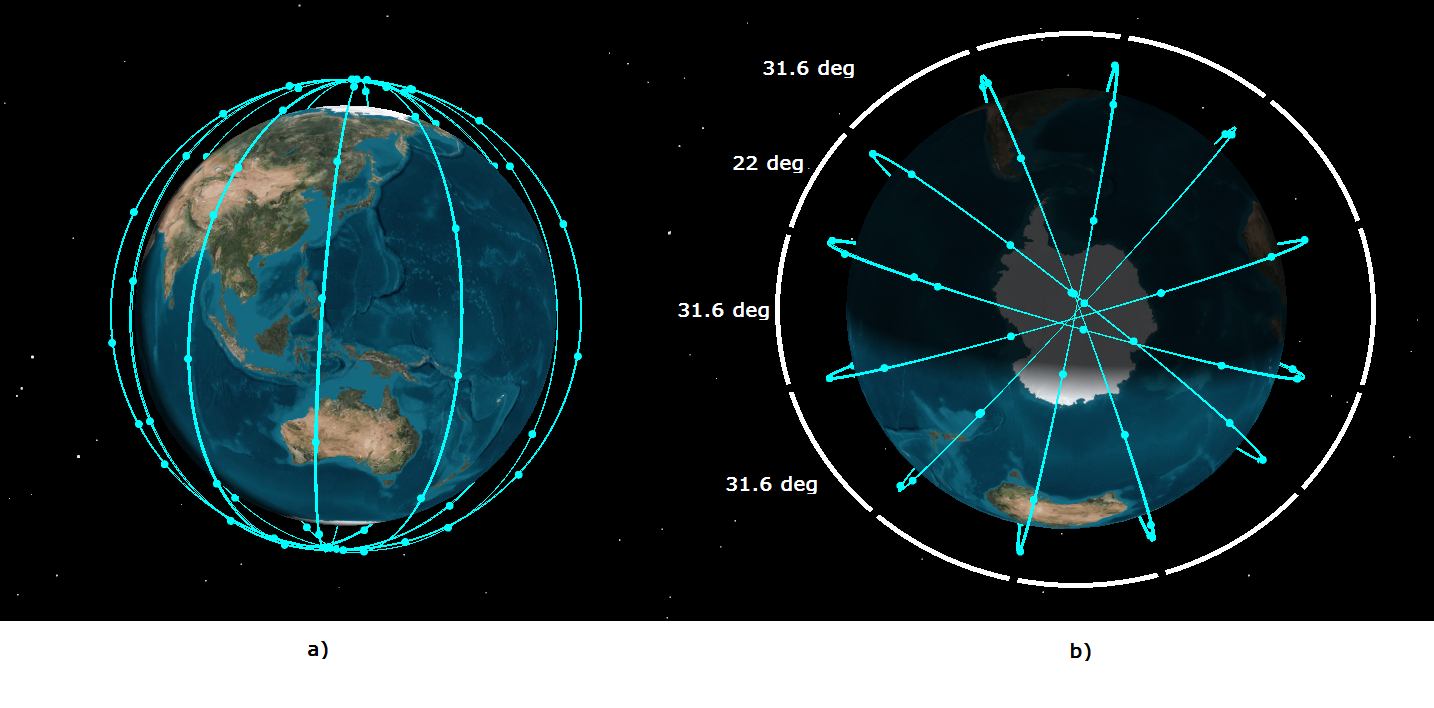
\includegraphics[scale = 0.35]{Pictures/iridium_stk.png}
	
	\caption{Iridium Satellite constellation showing a) a view over Australia and South East Asia and b) the view from above the south pole. Data taken from STK}
	\label{fig:iridium_stk}
\end{figure}
\begin{figure}[H]
	\centering
	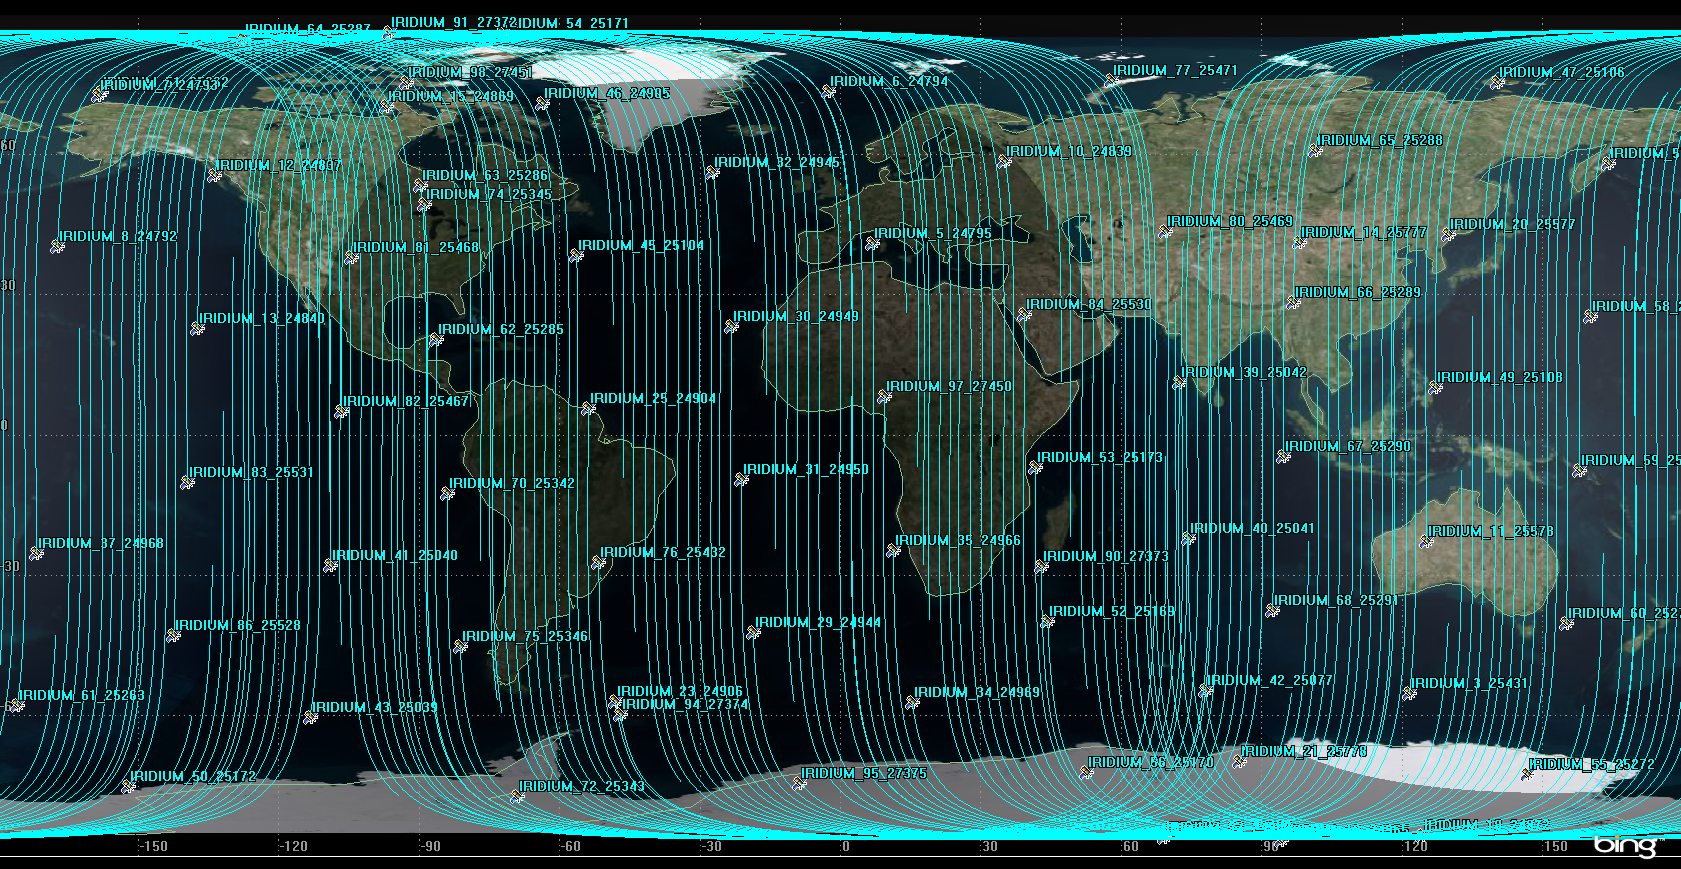
\includegraphics[scale = 0.20]{Pictures/iridium_2d_stk.png}
	
	\caption{Iridium Satellite constellation path over a 2D projection of the surface of the Earth. Data taken from STK}
	\label{fig:iridium_2d_stk}
\end{figure}

\subsubsection{Globalstar}
The Globalstar Constellation consists of 48 LEO satellites that provide mobile communication services that, as far as end-users are concerned, are much the same as those offered by Iridium, as detailed in Chapter \ref{sec:iridium}. Globalstar Inc. provide voice and data coverage over service areas where traditional PSTN data links are not availble. Unlike Iridium, Globalstar does not provide 100 percent global coverage, with swaths only covering areas between $70^\circ$ north and south latitudes \cite{Dietrich1998}.

The space segment of the Globalstar system consists of 48 satellites equally distributed in eight orbital planes. Each orbital plane contains 6 satellites has a $52^\circ$ inclination\cite{Smith1996, Dietrich1998}. Data from STK indicates that the orbits have equally spaced right ascensions of ascending node (RAANs) between $0^\circ$ and $360^ \circ$, offset $45^\circ$ from each other. Each satellite is in a roughly circular orbit, with an altitude of 1414 kilometres \cite{Smith1996} and a period of approximately 115 minutes. The eight orbital planes are illustrated in Figure \ref{fig:globalstar_stk}, with the ground track of all 48 satellites shown in Figure \ref{fig:globalstar_2d_stk}.
\begin{figure}[H]
	\centering
	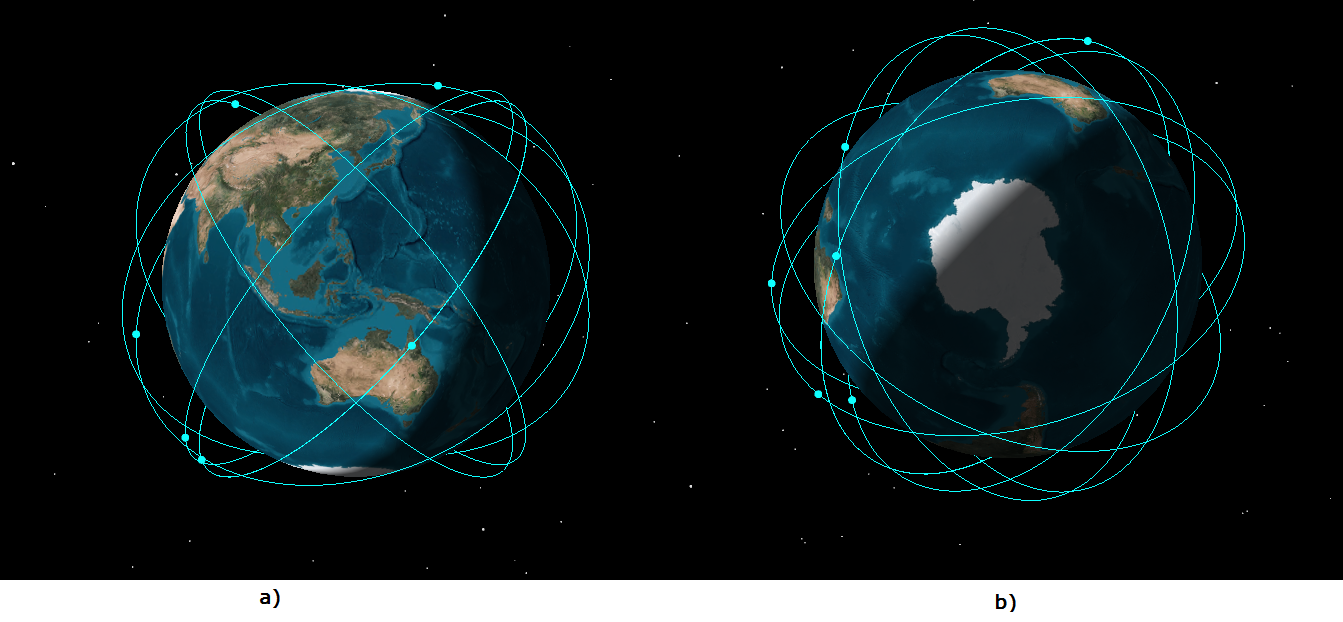
\includegraphics[scale = 0.40]{Pictures/globalstar_stk.png}
	
	\caption{The 8 Globalstar Orbital planes as shown from a) above Australia and South East Asia and b) above the south pole. Data from STK}
	\label{fig:globalstar_stk}
\end{figure}

\begin{figure}[H]
	\centering
	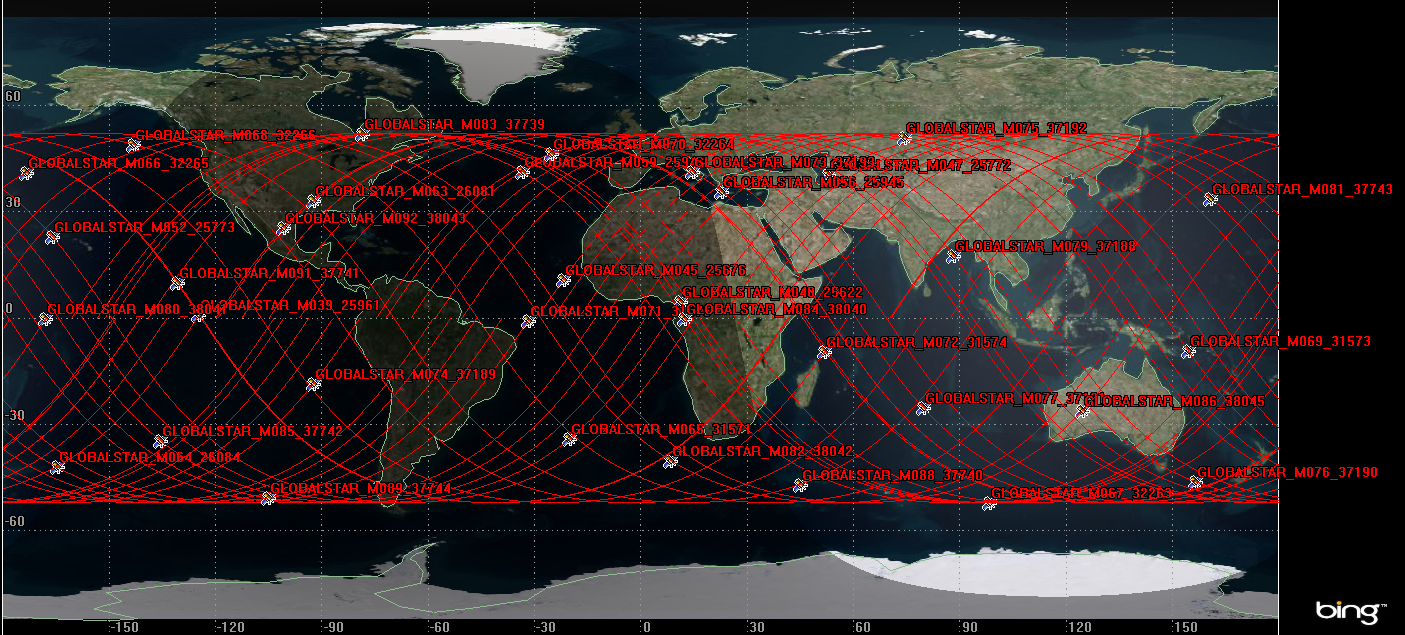
\includegraphics[scale = 0.40]{Pictures/globalstar_2d_stk.png}
	
	\caption{The Ground Track of the 48 Globalstar Satellites. Data from STK}
	\label{fig:globalstar_2d_stk}
\end{figure}

